%%
%% This is file `example/ch_intro.tex',
%% generated with the docstrip utility.
%%
%% The original source files were:
%%
%% install/buptgraduatethesis.dtx  (with options: `ch-intro')
%% 
%% This file is a part of the example of BUPTGraduateThesis.
%% 

\chapter{绪论}
\section{研究背景及意义}
随着互联网的发展,云数据中心的规模不断扩大,业务流量不断变化,如何为租户提供可编程的云数据中心网络,如何对云数据中心的流量进行有效的控制,提高带宽的利用率,降低成本,成为目前急需解决的问题。

软件定义网络(Software Defined Network,简称SDN) 作为一种新兴的可编程网络架构,有动态配置、可编程及快速响应的特点。其核心思想是将网络控制平面与数据转发平面分离,实现控制平面对数据平面的全局集中化控制;同时对外提供开放的可编程接口,为网络提供可编程能力。控制权的迁移使得底层构架能够抽象出来,各种应用和网络服务因此能将网络当作一个逻辑或虚拟实体,不再依赖于底层网络设备\cite{SDN-1},使得网络配置的自动化程度得到极大提高。通过应用SDN,除了网络的设计和操作变得简化,网络设备也得到简化,这些设备无需理解或处理成千上万的协议,只需要接受SDN控制器的指令即可。利用集中控制,网络管理员可以实时改变网络的行为,并且在几小时或几天内就可以部署新的应用和网络服务。

网络虚拟化\cite{Virtual-1}是一种将底层网络中的硬件以及配套的软件资源进行整合,形成统一管理实体的技术,通过虚拟网络资源到物理网络资源的映射,使得多个逻辑虚拟网络共享底层物理网络基础设施,为用户提供差异化服务。网络虚拟化技术是当今网络革新的重要技术之一。从概念上,网络虚拟化与SDN是互相独立的,但随着近几年网络技术的发展与融合,二者之间的联系变得越来越紧密,SDN的技术相关专题常会提及网络虚拟化技术,网络虚拟化问题的研究也时常会运用到SDN的概念,可见基于SDN的网络虚拟化技术已经成为网络技术研究领域的一个专门课题。

OpenStack\cite{Openstack-1}是由Rackspace和美国国家航空航天局(NASA)合作研发的用于搭建Iaas平台的云计算管理软件。旨在为公共及私有云的建设与管理提供软件的开源项目,主要提供计算、存储、网络服务。OpenStack支持几乎所有类型的云环境,项目目标是提供实施简单、可大规模扩展、丰富、标准统一的云计算管理平台。OpenStack通过各种互补的服务提供了基础设施即服务(IaaS)的解决方案,每个服务提供API以进行集成\cite{Openstack-2}。

在现有OpenStack云平台中,租户网络的创建与隔离仅限于服务器内部,OpenStack无法进行物理服务器之间数据中心网络的管控,跨服务器的通信通过隧道技术实现,该模式无法满足用户多样性的需求,同时无法实现云数据中心带宽资源的有效利用,时常会出现有些链路阻塞严重,而有些链路则处于空闲状态。

本文以此作为出发点,提出了一种多租户虚拟网络定制化管理方案,运用虚拟化技术,为租户提供相互隔离的虚拟SDN网络(简称vSDN),完成云数据中心物理资源有效利用的同时,虚拟SDN网络由租户自有的控制器实现集中管控,租户可以实时监测当前的流量状况并根据流量状况自定义转发路径,实现对网络的灵活管控,在不降低云平台性能的前提下,实现了OpenStack云平台中租户网络的定制化操作,既提高了安全性,又可以根据当下链路的剩余带宽,进行链路的定制化,提高带宽的利用率。对于租户本身而言,真正实现了租户对全局网络的可控性。对于运营商来说,对物理网络的集中控制可以大大较小网络配置的繁琐性,可以对网络故障实现快速的排查,提高可扩展性。

\section{主要研究内容及创新点}
\subsection{研究内容}

\subsection{创新点}
\section{研究生期间主要工作}
\section{论文组织结构}


\begin{enumerate}
\item 第二章介绍……
\item ……
\end{enumerate}
图\ref{fig:env1}
\begin{figure}[!htb]
  \centering
  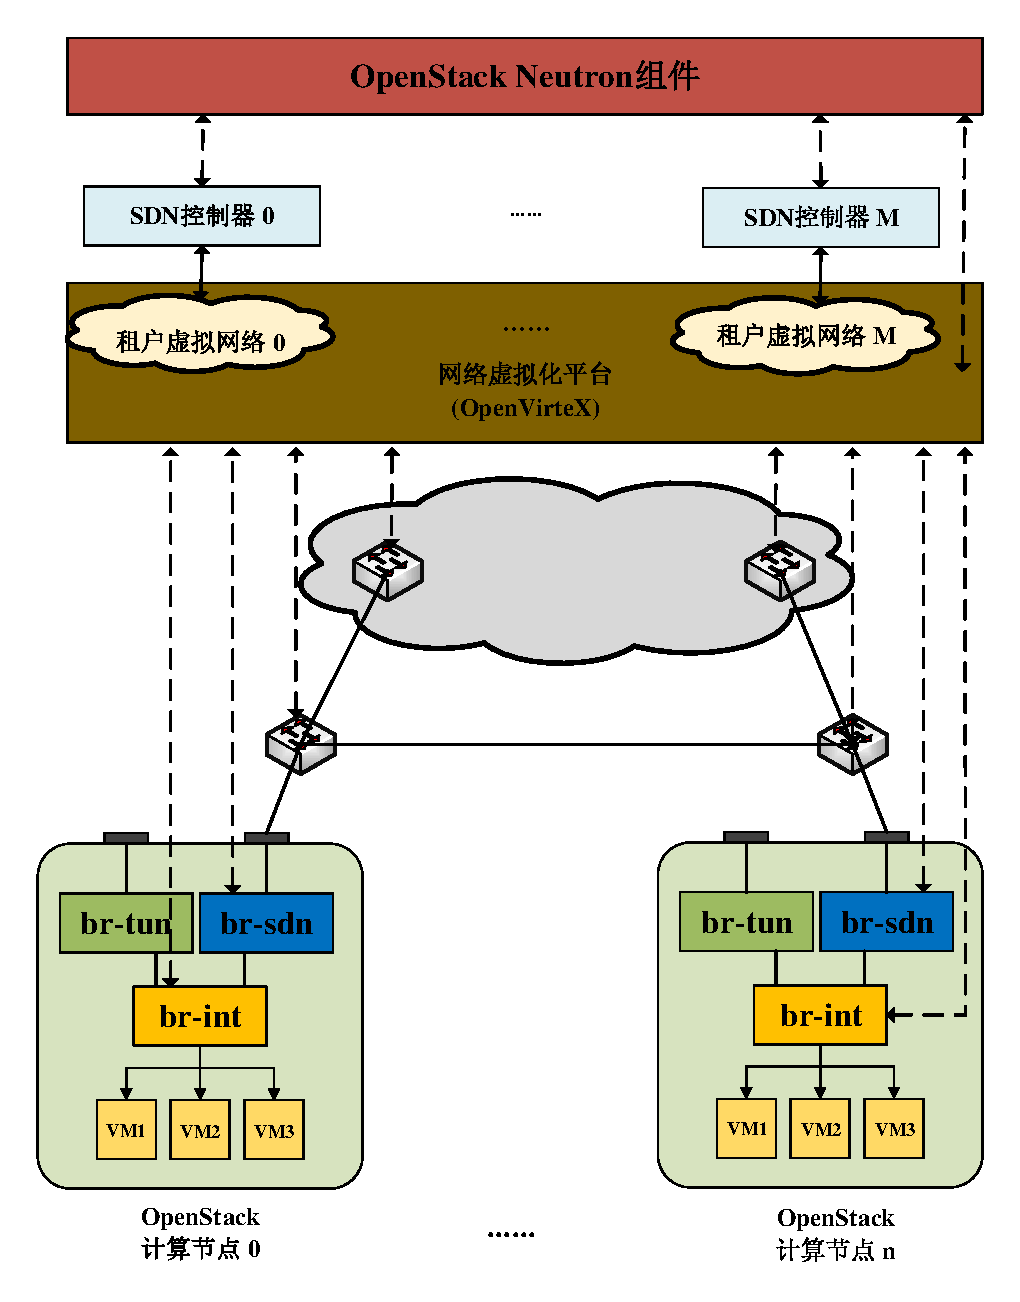
\includegraphics[width=100mm]{logo/architecture}
  \caption{System environment.}
  \label{fig:env1}
\end{figure}

%% 本章参考文献
\ifx\usechapbib\empty
\nocite{BSTcontrol}
\setcounter{NAT@ctr}{0}
\bibliographystyle{buptgraduatethesis}
\bibliography{bare_thesis}
\fi
